\section{Architectural styles}  

\begin{definition}[\textit{Architectural style}]
    An architectural style determines the vocabulary of components and connectors that can be used in instances of that style, together with a set of constraints on how they can be combined.
    These can include topological constraints on architectural descriptions (e.g., no cycles). 
    Other constraints—say, having to do with execution semantics—might also be part of the style definition.
\end{definition}

\subsection{Client-server}
The client-server architectural style is primarily employed in distributed applications, where the client initiates requests, and the server delivers responses.
\begin{figure}[H]
    \centering
    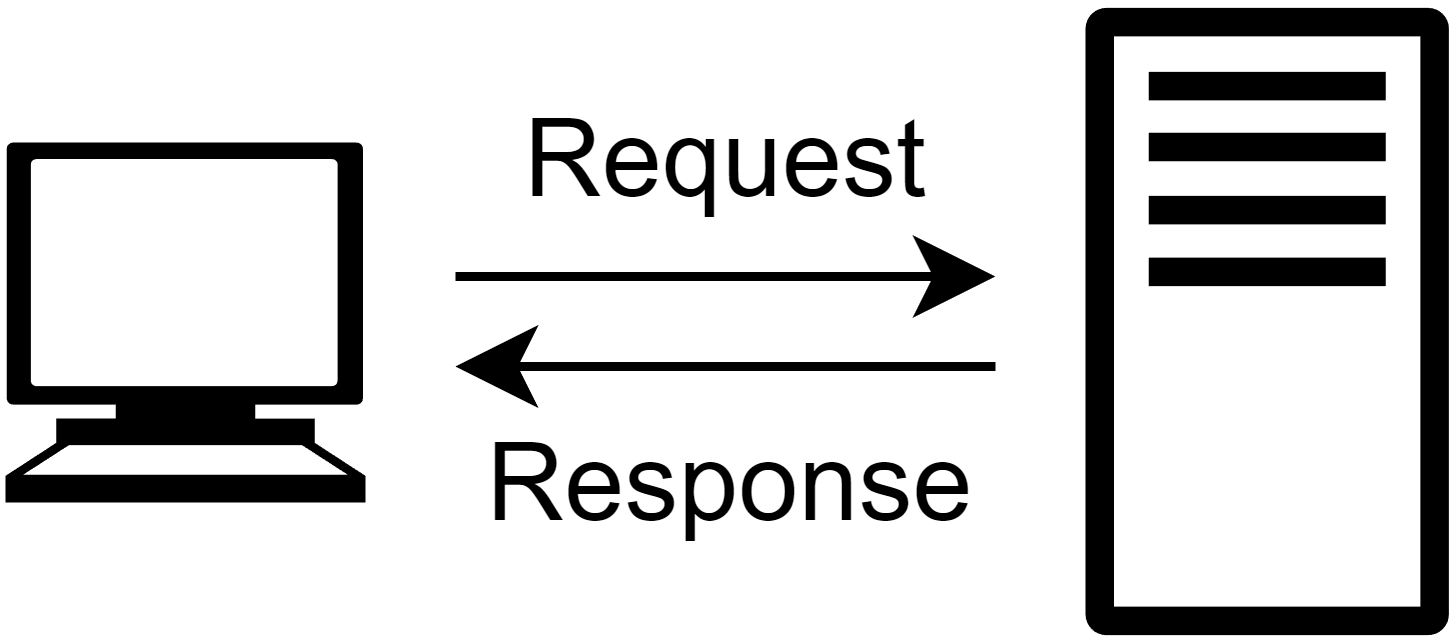
\includegraphics[width=0.35\linewidth]{images/clientserver.png}
    \caption{Client-server architecture general schema}
\end{figure}
This approach proves beneficial in situations where multiple users require access to a common resource, when there is a need to remotely access existing software, and when it is advantageous to structure the system around a shared functionality that multiple components utilize.
Key technical considerations for this architectural style include the design and documentation of well-defined interfaces for the server and the need to ensure the server's capability to handle concurrent requests efficiently.

In this architectural context, the requirement is to receive and manage requests from multiple clients. 
Various solutions can be considered to address this challenge:
\begin{itemize}
    \item \textit{Forking} (Apache Web Server): 
        \begin{itemize}
            \item Approach: create one process per request or per client.
            \item Strengths: simplicity, isolation, and protection provided by the one connection per process model. 
                Effective for up to 2000 users.
            \item Issues: limited capacity, uncertainty regarding the number of active processes at a given time, and scalability challenges due to the overhead of fork-kill operations.
        \end{itemize}
        \begin{figure}[H]
            \centering
            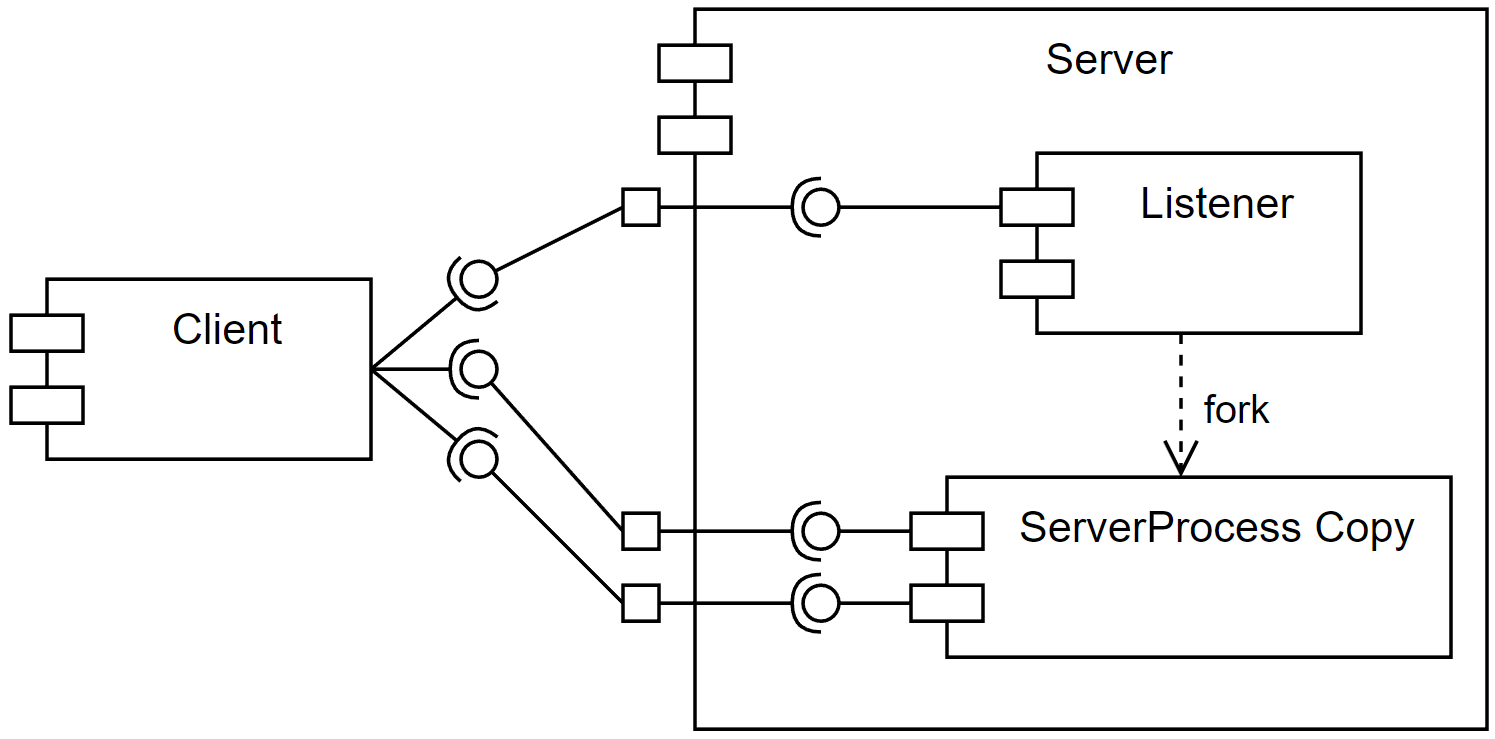
\includegraphics[width=0.5\linewidth]{images/fork.png}
        \end{figure}
        \begin{figure}[H]
            \centering
            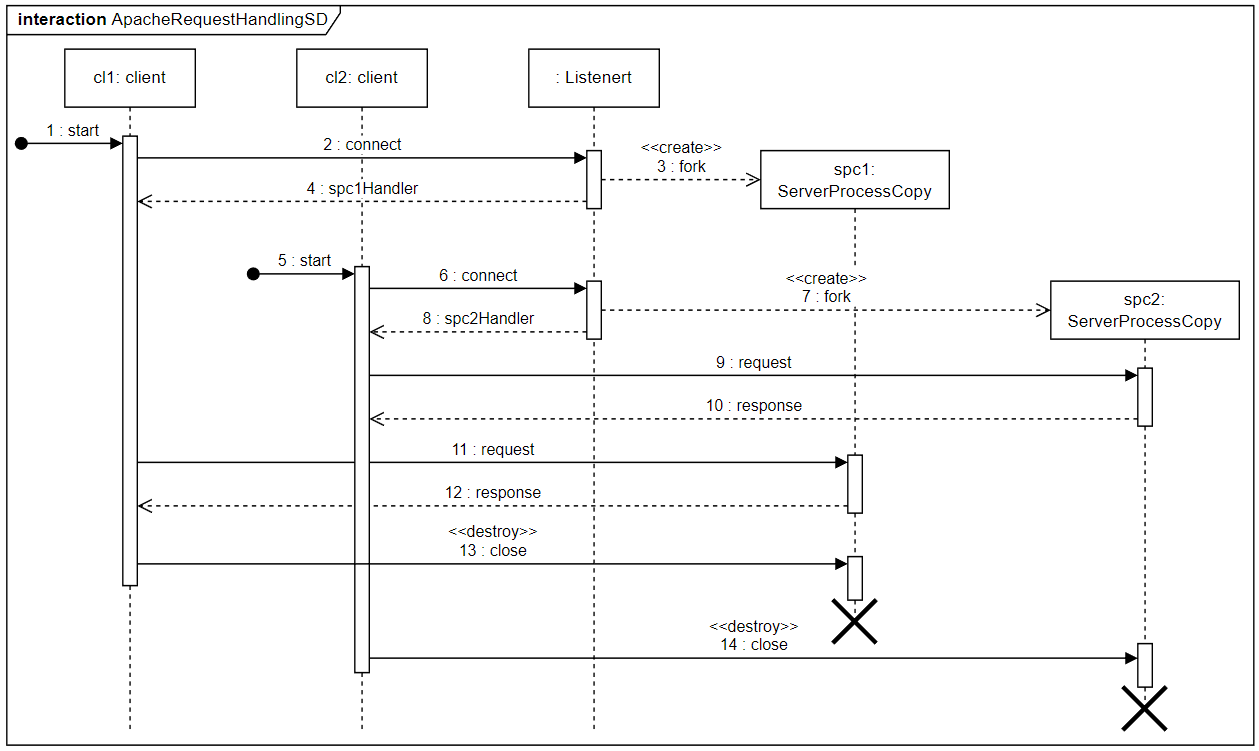
\includegraphics[width=0.7\linewidth]{images/fork1.png}
        \end{figure}
    \item \textit{Worker pooling} (NGINX Web Server): 
        \begin{itemize}
            \item Approach: specifically designed for high concurrency, addressing scalability issues inherent in the forking model by introducing a new architectural tactic.
            \item Architectural tactic: NGINX prioritizes scalability and performance at the expense of availability.
            \item Strengths: fixed number of workers for each pool, each worker equipped with a queue (with dropped requests for performance if the queue is full), and a dispatcher for load balancing among workers.
        \end{itemize}    
        \begin{figure}[H]
            \centering
            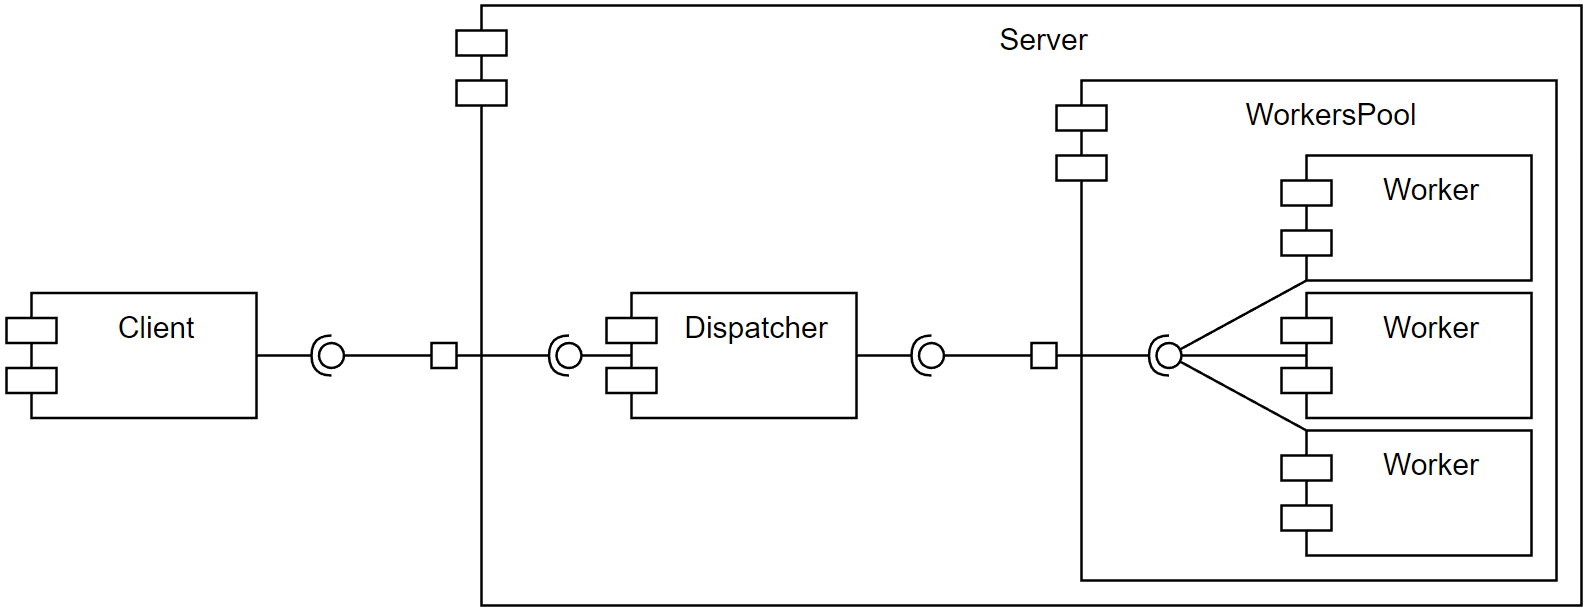
\includegraphics[width=0.5\linewidth]{images/work.png}
        \end{figure}
        \begin{figure}[H]
            \centering
            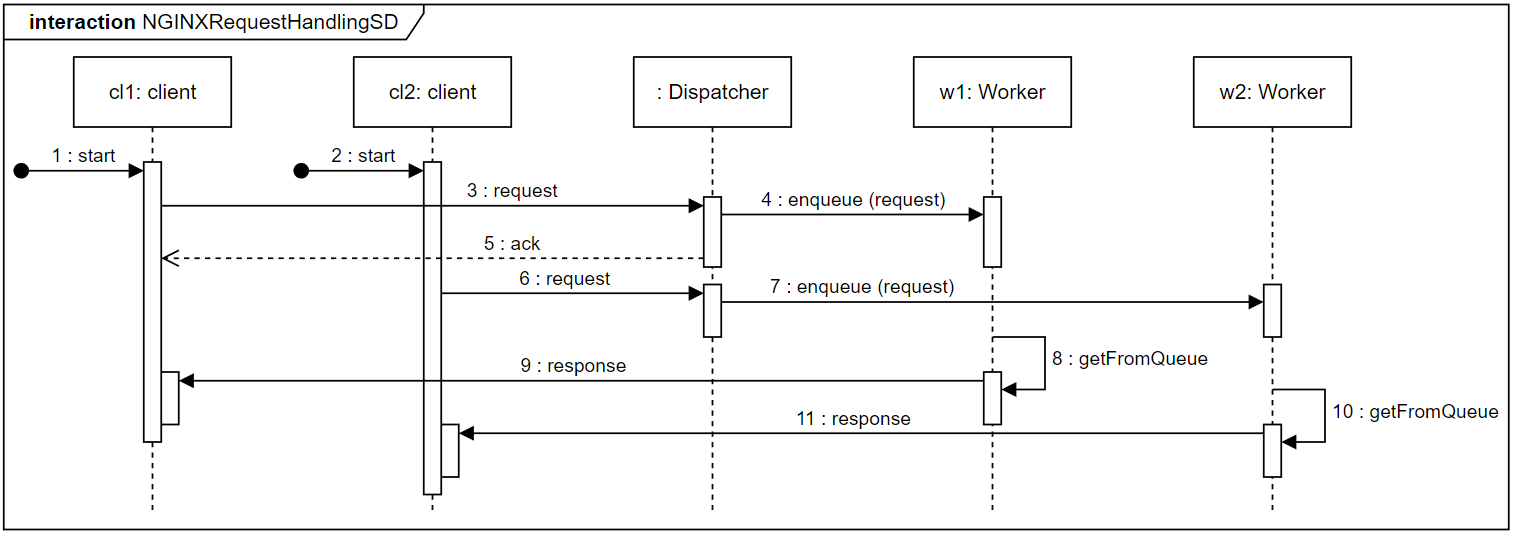
\includegraphics[width=0.9\linewidth]{images/work1.png}
        \end{figure}
\end{itemize}

\subsection{Three-tier architecture}
Within three-tier architectures, the intermediate tier is responsible for handling the application logic. 
The primary advantage lies in the separation of logic from both data and presentation elements. 
The modular structure allows for enhanced flexibility and maintainability.

With the option of incorporating additional tiers, it becomes feasible to establish an N-tier architecture. 
This extended architecture enables further refinement and specialization of components, supporting more intricate and scalable system designs.

\subsection{Event-driven architecture}
In an event-driven architecture, components can register to both send and receive events that are broadcasted to all registered components, where neither the sender nor the receiver is known.
This model, often referred to as publish-subscribe, facilitates easy addition and deletion of components and is increasingly employed in modern integration strategies.
Key characteristics include asynchronous events, reactive computation, message destination determined by the receiver, loose coupling, and flexible communication means.
Strengths and challenges of this architecture include its widespread adoption in modern development practices, ease of adding and removing components, potential scalability issues, and complexities in event ordering.

Apache Kafka serves as a framework for the event-driven paradigm, providing primitives for creating event producers and consumers, along with a runtime infrastructure for handling event transfer. 
Kafka stores events durably and reliably, allowing consumers to process events in real-time or retrospectively. 
These services are delivered in a distributed, highly scalable, elastic, fault-tolerant, and secure manner.
\begin{figure}[H]
    \centering
    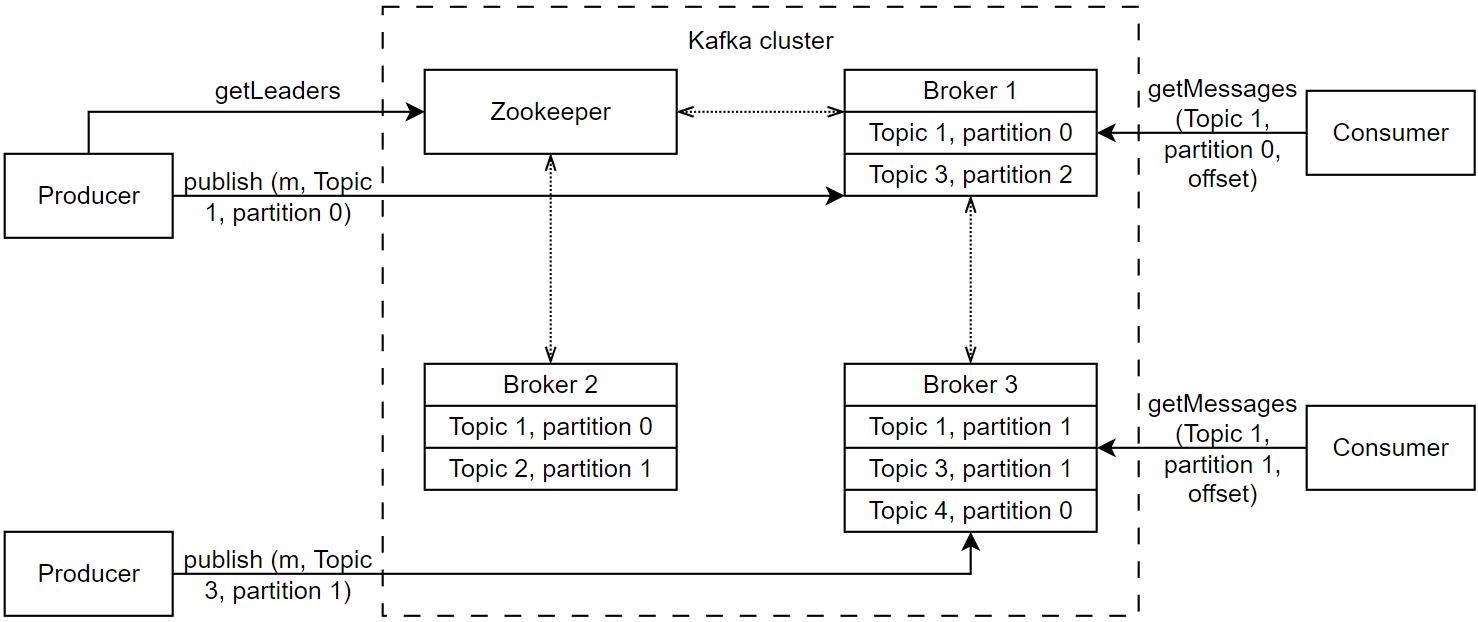
\includegraphics[width=0.75\linewidth]{images/kafka.png}
\end{figure}
The Kafka architecture involves brokers managing designated topics and partitions, with each partition containing sets of messages related to the respective topic. 
The partitions operate independently and can be duplicated across multiple brokers to ensure fault tolerance.

Each partition designates one broker as the leader, while the remaining brokers hosting the same partition act as followers. 
Producers are aware of the leading brokers and direct their messages to them. 
Messages within a given topic are grouped into batches on the producer's end and transmitted to the broker once the batch size surpasses a specified threshold.

Consumers employ a pull mechanism, retrieving an entire batch of messages associated with a specific partition from a defined offset. 
Messages persist at the broker level for a predetermined duration and can be accessed multiple times during this period.

The leader broker keeps tabs on the in-sync followers. 
The correct functioning of the cluster is overseen by ZooKeeper, with all brokers regularly sending heartbeats to it. 
In the event of a broker failure, ZooKeeper intervenes by appointing a new leader for all partitions previously led by the failing broker. 
Additionally, ZooKeeper has the capability to initiate or restart brokers as needed.

Brokers finalize message commitment by storing them in their designated partition. 
The leader includes the message in the followers (replicas) if they are accessible. 
A potential challenge arises in the event of failure, where the producer may not receive a response, as illustrated by message seven. 
Consequently, the producer is required to resend the message.

Kafka brokers possess the ability to recognize and eliminate duplicate messages. 
The synchronization process with replicas can be transactional, allowing for precise control over the message flow. 
Achieving exactly-once semantics is feasible but comes with the trade-off of longer waiting times. 
Alternatively, opting for at-least-once semantics involves excluding duplicate management, and at-most-once semantics can be chosen by dispatching messages asynchronously.
\begin{figure}[H]
    \centering
    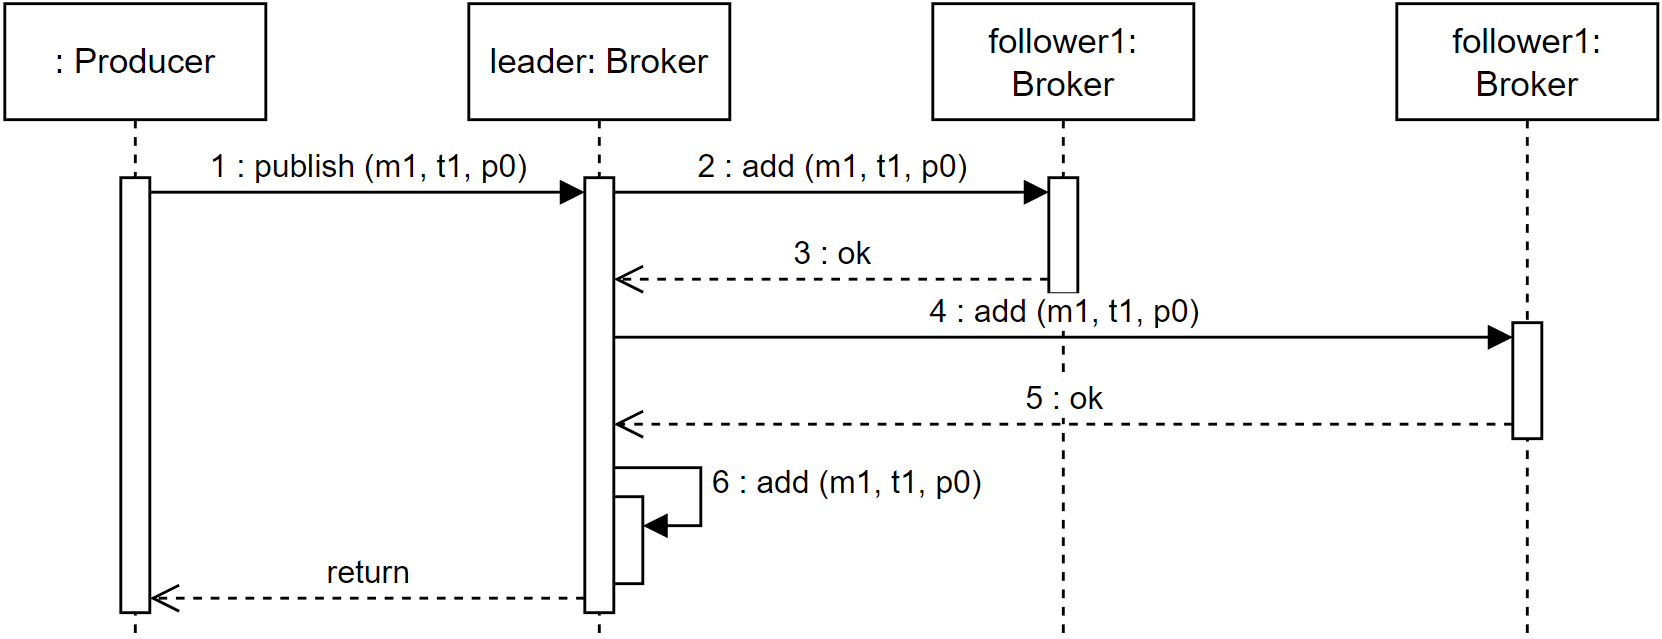
\includegraphics[width=0.75\linewidth]{images/producer.png}
    \caption{Example of a producer}
\end{figure}

Every consumer has access to a persistent log to maintain the offset, ensuring it is preserved in the event of a failure. 
If a consumer encounters a failure after processing messages but before recording the new offset in the log, it will retrieve the same messages again, resulting in at-least-once semantics.

The delivery semantics can be altered by storing the new offset before processing. 
In this case, if a failure occurs after storing the offset, the impact of the received messages does not materialize, leading to at-most-once semantics.

Transactional management of the log introduces the capability for exactly-once semantics, providing a robust mechanism for ensuring that each message is processed only once, even in the face of failures or system disruptions.
\begin{figure}[H]
    \centering
    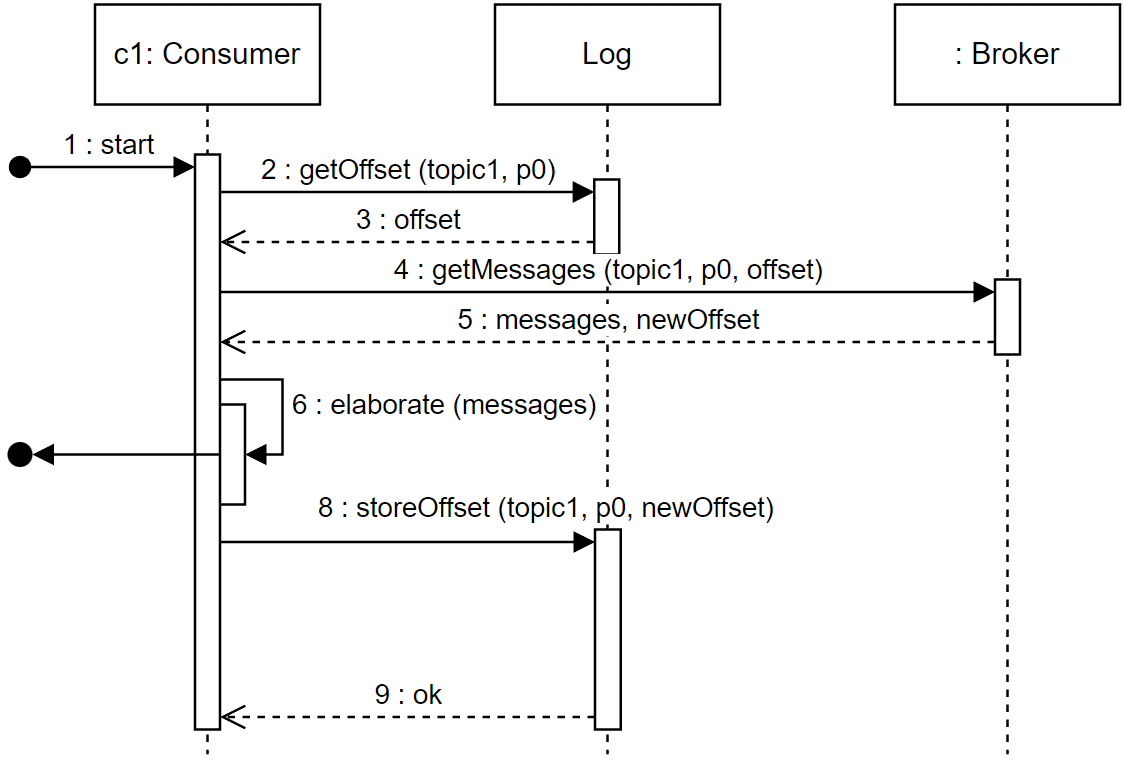
\includegraphics[width=0.75\linewidth]{images/consumer.png}
    \caption{Example of a consumer}
\end{figure}
Apache Kafka's architectural tactics include scalability through multiple partitions and brokers and fault tolerance through persistent partition storage and data replication.

\subsection{Microservices}
In the era preceding microservices, monolithic systems delivered applications as single deployable software artifacts. 
The microservice architectural style emerged as an approach to developing applications by decomposing monolithic systems into small, specialized services, each running independently in its own process. 
These services communicate using lightweight mechanisms, often employing HTTP resource APIs.

Microservices focus on addressing a single bounded context within the target domain, offering advantages such as fine-grained scaling strategies, reduced impact of localized issues, improved resilience through decentralized functionality, and enhanced reuse and composability.

The process of creating a microservices architecture involves reducing teams' synchronization overhead, organizing small development teams with well-defined responsibilities, and employing technology-neutral protocols like REST APIs for communication, resulting in smaller codebases for easier debugging and more cost-effective maintenance.

The architecture's main elements include a REST API that exposes core service operations, the application or business logic responsible for implementing core operations, and local data storage for each microservice, emphasizing limited data sharing and avoiding global databases.

The standard process in a microservice architecture involves the following steps:
\begin{enumerate}
    \item A client initiates an HTTP GET request to the Hello microservice.
    \item The microservice parses the HTTP request, mapping the verb, URL, resource, and parameters to a corresponding method in the codebase.
    \item After identifying the route, the microservice maps any defined parameters within the route to arguments of the associated method.
    \item Additional parameters can be transmitted through JSON in the HTTP body, mapping to objects utilized by the method.
    \item Once the data is mapped, the microservice executes the business logic, which may involve calling operations exposed by other microservices.
    \item After the execution of business logic, the microservice converts the returned objects into JSON.
    \item The client receives the response from the microservice in JSON format, with the success or failure of the call indicated by the HTTP status code.
\end{enumerate}

To achieve location transparency and scalability in microservices, routing patterns are essential.
Service discovery, a critical element, must be highly available, load-balanced, resilient, and fault-tolerant. 
Resilience patterns, such as the circuit breaker pattern, aim to prevent resource waste and ripple effects by actively monitoring calls to distant services and intervening in case of potential failures.
\begin{figure}[H]
    \centering
    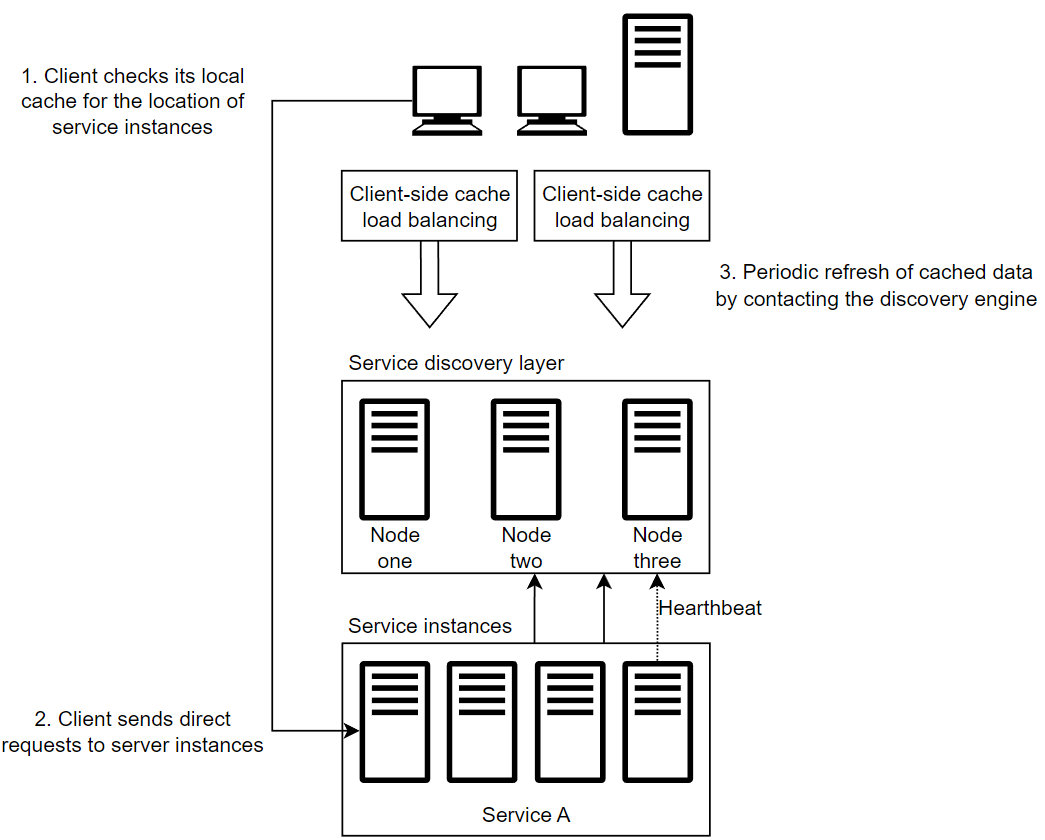
\includegraphics[width=0.75\linewidth]{images/rp.png}
    \caption{Routing pattern}
\end{figure}

To allow the microservices to be resilient we need resiliency patterns. 
The main goal of these patterns are to avoid useless resource consumption and ripple effects. 
Circuit breaker is a client-side resiliency pattern. 
The circuit breaker functions as a proxy for a distant service. 
As it invokes the remote service, the CB actively monitors the call for potential failures, which may include receiving a 5xx error or the call taking an excessively long duration, prompting the CB to terminate the call.
In the event of "too many" failures, the circuit breaker intervenes by inhibiting future calls to prevent further issues.
\begin{figure}[H]
    \centering
    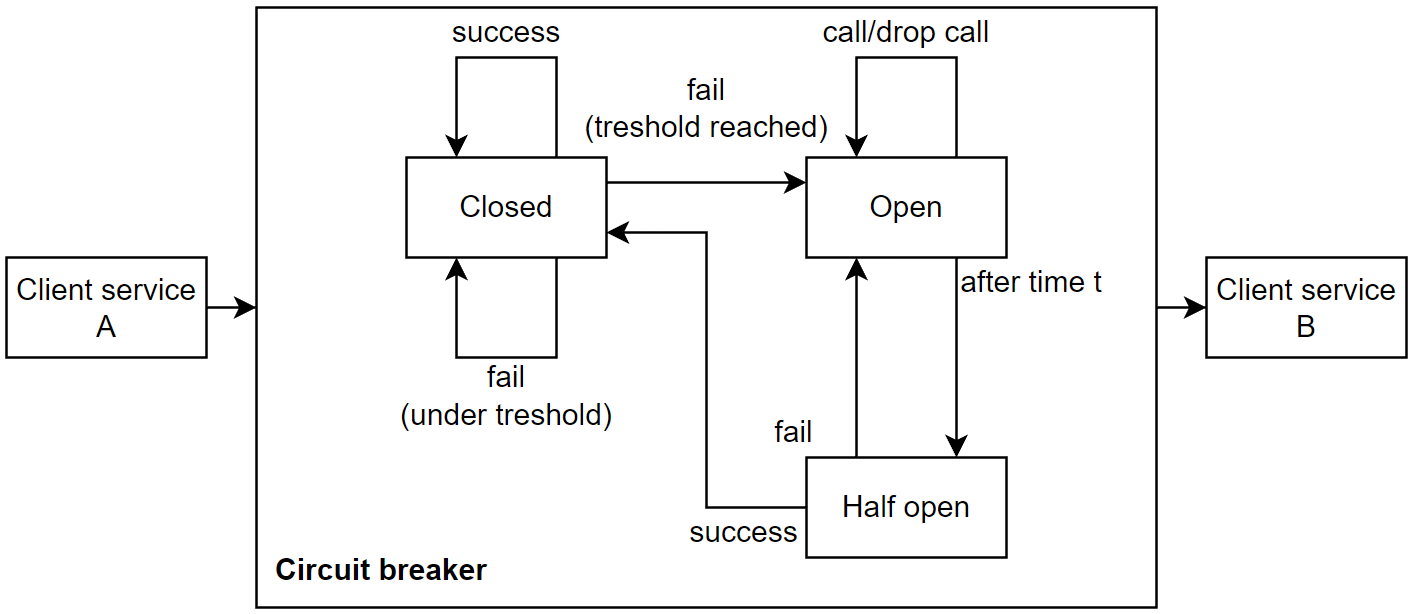
\includegraphics[width=0.75\linewidth]{images/cb.png}
    \caption{Circuit breaker pattern}
\end{figure}

Security patterns in microservices involve introducing a service or API gateway that acts as a mediator between service clients and invoked services. 
While this gateway simplifies the implementation of authentication and authorization mechanisms, it can become a single point of failure. 
This challenge is mitigated by deploying multiple instances of the gateway with a server-side load balancer.
\begin{figure}[H]
    \centering
    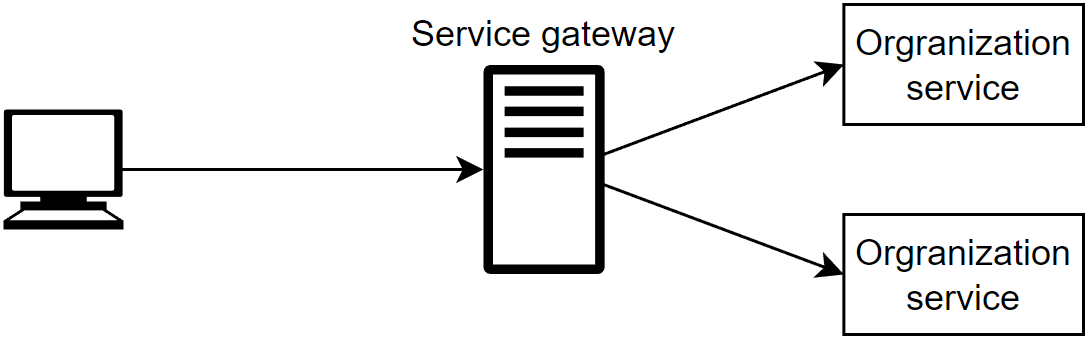
\includegraphics[width=0.5\linewidth]{images/sp.png}
    \caption{Security pattern}
\end{figure}

Communication patterns play a crucial role in achieving loose coupling in microservices. 
Despite their strengths in providing flexibility, scalability, and availability, they introduce higher complexity. 
Event-driven frameworks, supporting multiple communication styles such as notification, request/response, and publish/subscribe, are employed to decouple different parts of the system.
\begin{figure}[H]
    \centering
    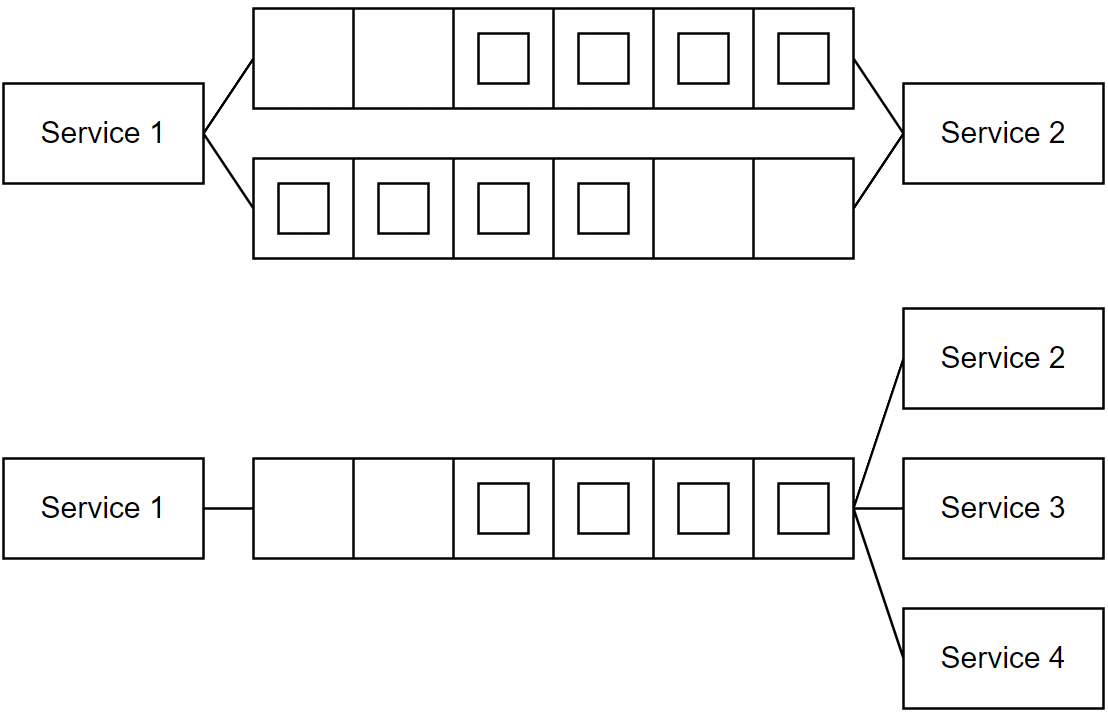
\includegraphics[width=0.75\linewidth]{images/cp.png}
    \caption{Security pattern}
\end{figure}
\newpage